\documentclass[a4, 12pt]{article}
\usepackage[a4paper,top=1.3cm,bottom=2cm,left=1.5cm,right=1.5cm,marginparwidth=0.75cm]{geometry}
\usepackage{setspace}
\usepackage{cmap}
\usepackage{mathtext}
\usepackage[utf8]{inputenc}
\usepackage[english,russian]{babel}
\usepackage[T2A]{fontenc}
\usepackage{multirow}
\usepackage{graphicx}
\usepackage{wrapfig}
\usepackage{tabularx}
\usepackage{float}
\usepackage{longtable}
\usepackage{hyperref}
\hypersetup{colorlinks=true,urlcolor=blue}
\usepackage[rgb]{xcolor}
\usepackage{amsmath,amsfonts,amssymb,amsthm,mathtools}
\usepackage{icomma}
\mathtoolsset{showonlyrefs=true}
\usepackage{euscript}
\usepackage{mathrsfs}
\usepackage{array}
\usepackage{caption}
\usepackage{eqnarray}



\title{Фазовые переходы I рода. Уравнение Клапейрона-Клаузиуса}
\author{Дудаков Семён, группа Б01-303}
\date{}

\begin{document}
	\maketitle
\section{Введение}
{\itshape\textbf{\space\space\spaceФаза}} — это физически однородная
часть системы, отличающаяся своими физическими свойствами от
других частей и отделенная от них четко выраженной границей.
Фазы могут контактировать друг с другом, находясь в равновесии.
Примерами являются двухфазные системы:
\begin{enumerate}
    \item «жидкость–пар» (например, «вода–пар»)
    \item «жидкость–твердое тело» (например, «вода–лед»)
    \item две различные кристаллические модификации одного и того же
вещества, находящиеся в контакте
\end{enumerate}
\par
{\itshape\textbf{Фазовым переходом}} называется переход вещества из одной фазы
в другую при изменении внешних условий (температуры, давления,
электрического и магнитного полей), при подводе или отводе тепла
и т. д.
\par
{\itshape\textbf{Экстенсивная величина}} — пропорциональная объёму подсистемы.
Имеется в виду следующее. Пусть имеется некоторая экстенсивная
величина $X$. Мысленно разделим систему на $n$ макроскопических
частей, так что для $i$-й подсистемы рассматриваемая величина принимает значение $X_i$. Тогда для всей системы $X=\sum_{i=1}^{n} X_i$. 
\parПримеры: объем $V$ , внутренняя энергия $U$, энтропия $S$.
\parВеличины, не зависящие от объема выделенной подсистемы, называются {\itshape\textbf{интенсивными}}. Примеры: температура $T$, давление $P$ , плотность $\rho$.
\par
{\itshape\textbf{Химический потенциал μ}}— это
величина, определяющая изменение энергии системы при добавлении одной частицы вещества:
\begin{equation}
    dU = TdS - P dV + \mu dN, \mu = \left(\frac{\partial U}{\partial N}\right)_{S,V}
\end{equation}
где N — число частиц в системе. Справедливо также соотношение:
\begin{equation}
    d\Phi = - SdT + VdP + \mu dN
\end{equation}
Интенсивные величины не зависят от числа частиц в системе, а
экстенсивные пропорциональны этому числу. В частности, это означает, что:
\begin{equation}
    \Phi = \Phi(T, P, N) = Nf(T, P)
\end{equation}
Из последнего соотношения следует:
\begin{equation}
    \mu = \left(\frac{\partial\Phi}{\partial N} \right)_{P, T}=\frac{\Phi}{N}
\end{equation}
\parТаким образом, химический потенциал $\mu = \mu(P, T)$ есть термодинамический потенциал в расчете на одну частицу. Поскольку $d\Phi = -Sdt + VdP + \mu dN$ и $\Phi = \mu N$ , то
$d\mu = -sdT+vdP$,
где $s =\frac{S}{N}, v = \frac{V}{N}$ — энтропия и объем в расчете на одну частицу. Химический потенциал μ — интенсивная величина.
\section{Условие равновесия фаз}
\begin{wrapfigure}{r}{0.5\textwidth}
           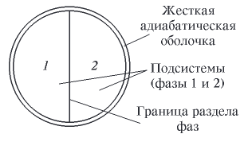
\includegraphics[width=1\linewidth]{vpv1.png} 
           \caption{}
           \label{ris:image}
\end{wrapfigure}
\ \ \ \ Рассмотрим двухфазную систему «1 + 2», помещенную в жесткую адиабатическую оболочку (см. рис.1).
\parПроведем в системе некоторый
бесконечно малый процесс, в ходе
которого фазы находятся в тепловом
и механическом равновесии:
\begin{equation}
    T_1 = T_2 = T, \ P_1 = P_2 = P.
\end{equation}
Тогда изменения внутренней энергии фаз 1 и 2 будут равны:
\begin{eqnarray}
    dU_1 = TdS_1 - PdV_1 + μ_1dN_1\\
    dU_2 = TdS_2 - PdV_2 + μ_2dN_2
\end{eqnarray}
Сложим почленно эти равенства. Введем полную энтропию системы $S = S_1 + S_2$.Вследствие изолированности системы ее энергия сохраняется: $dU_1 = −dU_2$, а неизменность полного объема системы влечетза собой равенство $dV_1 = −dV_2$. Поэтому:
\begin{equation}
    TdS + \mu_1dN_1 + \mu_2dN_2 = 0
\end{equation}
Поскольку полное число молекул вещества не меняется, то $dN_1 = −dN_2$. Следовательно, изменение полной энтропии системы в результате процесса определится из соотношения
\begin{equation}
    TdS = (\mu_1 - \mu_2)dN_2
\end{equation}
В состоянии термодинамического равновесия энтропия имеет максимум, т. е. dS = 0 и из последнего равенства следует
\begin{equation}
    \mu_1 = \mu_2
\end{equation}
\section{Уравнение Клапейрона-Клаузиуса}
\begin{wrapfigure}{r}{0.5\textwidth}
           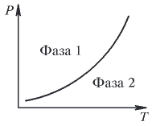
\includegraphics[width=0.8\linewidth]{vpv2.png} 
           \caption{}
           \label{ris:image}
\end{wrapfigure}
\ \ \ \ В состоянии равновесия двух фаз выполняется равенство $\mu_1(P, T) = \mu_2(P, T)$, где индексы 1 и 2 относятся к различным фазам одного вещества. Отсюда следует $P = P(T)$. Это значит, что фазы могут сосуществовать, если только давление и температура в системе удовлетворяют указанному соотношению, т. е. лежат на {\itshape\textbf{кривой фазового равновесия}} (см. рис. 2). 
\parНайдем дифференциальное уравнение кривой фазового равновесия. При изменении Т и P выполняются равенства:
\begin{eqnarray}
    d\mu_1 = -s_1dT + v_1dP\\
    d\mu_2 = -s_2dT + v_2dP
\end{eqnarray}
Поскольку $\mu_1(P, T) = \mu_2(P, T)$, то $d\mu_1 = d\mu_2$, откуда следует:
\begin{equation}
    (s_2 - s_1)dT = (v_2 - v_1)dP \text{\ или \ }  \frac{dP}{dT} = \frac{s_2 - s_1}{v_2 - v_1}
\end{equation}
\newpage
Введем обозначение: $q_{12} = T(s_2 - s_1)$. Тогда последнее уравнение примет вид:
\begin{equation}
    \frac{dP}{dT} = \frac{q_{12}}{T(v_2 - v_1)} 
\end{equation}
Это соотношение называется {\itshape\textbf{уравнением Клапейрона–Клаузиуса}}.
\parВеличина $q_{12}$ называется теплотой фазового перехода 1 → 2 (в
расчете на одну частицу) и имеет смысл энергозатрат на осуществление перехода. Если в фазовом переходе тепло поглощается, то $q_{12}$ > 0.
Если же тепло выделяется, то $q_{12}$ < 0.
\section{Фазовые переходы первого рода}
\ \ \ \ Фазовыми переходами первого рода называются такие переходы, при которых скачком меняются первые производные химического потенциала $\mu(P, T)$. Поскольку:
\begin{equation}
    v = \left(\frac{\partial\mu}{\partial P}\right)_T, \
    s = -\left(\frac{\partial\mu}{\partial T}\right)_P
\end{equation}
То значит, что при этих переходах скачкообразно меняется плотность вещества $(\rho \sim v^\text{-1})$. Кроме того, отлична от нуля теплота фазового перехода
$q_{12} = T(s_2 - s_1)$.
\parПримеры: плавление, испарение, возгонка и обратные им
\section{Заключение}
\ \ \ \ В ходе проделанной работы были изучены явления фазового перехода, рассмотрены экстенсивные и интенсивные величины. Для вывода уравнения фазового перехода был введён, так назыаемый, химический потенциал, являющийся интенсивной величиной. Было получено условие равновесия фаз, а из него практически сразу получилось уравнение Клапейрона-Клаузиуса. Были рассмотрены фазовые переходы первого рода.
\section{Список использованной литературы}
\begin{enumerate}
    \item Д.В. Сивухин, Общий курс физики, Том2 - Термодинамика и молекулярная физика
    \item Н.А. Кириченко, Термодинамика, статистическая и молекулярная физика
\end{enumerate}
\end{document}
